\section{What we discussed last time}
\subsection{Parsing}
\begin{frame}[fragile]{Parsing}
	
	\begin{columns}[T,onlytextwidth]
		
		% LEFT COLUMN: lstlisting
		\begin{column}{0.46\textwidth}
		\boxtext{Crystallization was carried out in sitting-drop vapor-diffusion setups with 1:1 mixtures of protein solution containing 0.7 M hepes and 1.8 M MnCl2 and reservoir solution containing 19--21\% PEG 3350 and 30\% polyethylene glycol monomethyl ether 4000 and 0.2 M Na2HPO4, pH 9.5, VAPOR DIFFUSION, SITTING DROP, temperature 298K.}
		\end{column}
		
		
		% RIGHT COLUMN: boxtext
		\begin{column}{0.5\textwidth}
			
			\begin{verbatim}
				{
					"protein": {
						"hepes": "700 mM",
						"MnCl2": "1800 mM"
					},
					"reservoir": {
						"PEG 3350": "20%",
						"PEGMME 4000": "30%",
						"Na2HPO4": "200 mM"
					},
					"pH": 9.5,
					"temperature": "298 K"
				}
			\end{verbatim}
		\end{column}
		
		
	\end{columns}
	
\end{frame}

\subsection{Data Analysis}
\begin{frame}{Data Analysis}
	\begin{figure}[h!]
		\centering		
		\begin{subfigure}[t]{0.495\linewidth}
			\centering
			\includegraphics[width=\linewidth]{../../msc-thesis-code/data/dataExploration/plots/surface_entropy_fraction_VsChem}
			\label{fig:surface_entropy_fractionVsChem}
		\end{subfigure}
		\begin{subfigure}[t]{0.495\linewidth}
			\centering
			\includegraphics[width=\linewidth]{../../msc-thesis-code/data/dataExploration/plots/2d_hist_plot}
			\label{fig:2d_hist_plot}
		\end{subfigure}	
		\label{fig:distribution_analysis}
	\end{figure}
	
\end{frame}

\section{What has changed since then}
\subsection{Additional feature}
\begin{frame}{Additional Feature}
	\begin{figure}[h]
		\centering		
		\begin{subfigure}[t]{0.40\linewidth}
			\centering
			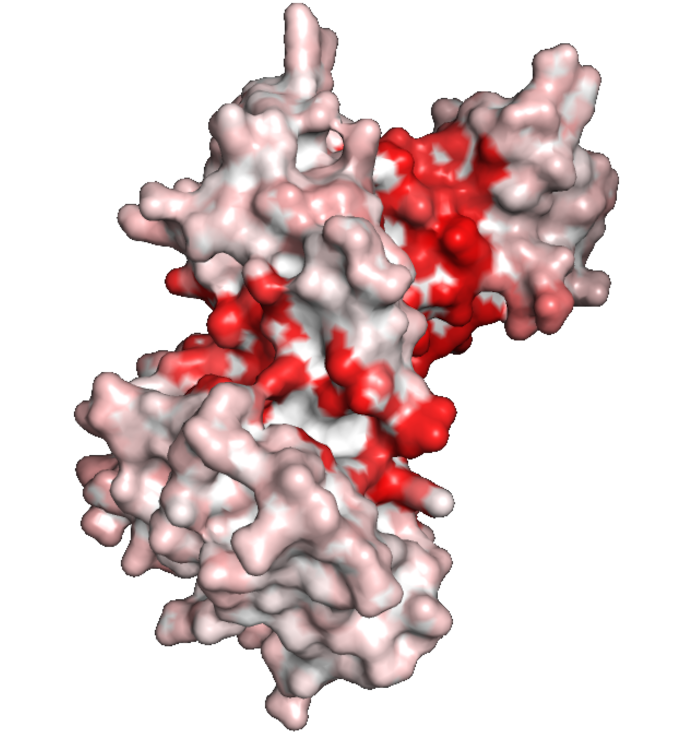
\includegraphics[width=\linewidth]{media/binding_site9ewo}
		\end{subfigure}
		\begin{subfigure}[t]{0.40\linewidth}
			\centering
			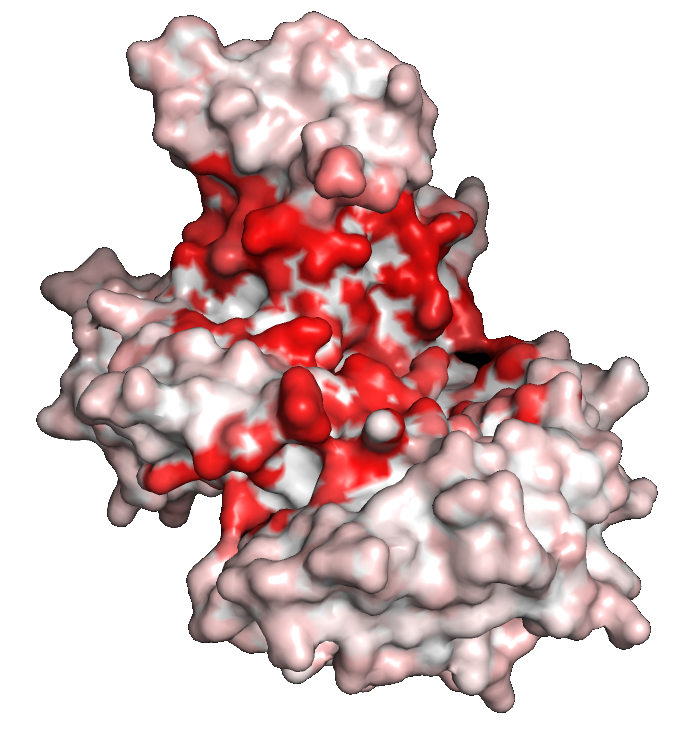
\includegraphics[width=\linewidth]{media/binding_site2fz3}
		\end{subfigure}
		\label{fig:bindingSitePrediction}
	\end{figure}
\end{frame}

\subsection{Misspellings}
\begin{frame}{Misspellings}
	
	\begin{columns}[T,onlytextwidth]		
		% LEFT COLUMN: lstlisting
		\begin{column}{0.3\textwidth}
			\begin{itemize}
				\item normalized Levenshtein ratio to find mispellings
				\item >90\% (ammonia vs. ammonium)
				\item further filtering: disodium malonate/sodium malonate or hexanediol/heptanediol
				\item removes 30\% of unique chemical names
			\end{itemize}			
		\end{column}
		
		
		% RIGHT COLUMN: boxtext
		\begin{column}{0.69\textwidth}			
			\begin{figure}
				\centering
				\includegraphics[width=1.1\linewidth]{../../msc-thesis-code/data/dataExploration/plots/coverageByThreshold}
			\end{figure}
		\end{column}		
		
	\end{columns}	
\end{frame}

\subsection{Chemical dependent difficulty}
\begin{frame}{Find the crux}
	\begin{figure}[h!]
		\centering		
		\begin{subfigure}[t]{0.495\linewidth}
			\centering
			\includegraphics[width=\linewidth]{../../msc-thesis-code/data/dataExploration/plots/ks_distance_all_sequence}
			\label{fig:ks_distance_all_sequence}
		\end{subfigure}
		\begin{subfigure}[t]{0.495\linewidth}
			\centering
			\includegraphics[width=\linewidth]{../../msc-thesis-code/data/dataExploration/plots/ks_distance_all}
			\label{fig:ks_distance_all_surface}
		\end{subfigure}
		\label{fig:ks_distance_all_features}
	\end{figure}
\end{frame}

\subsection{Condition Embedding}
\begin{frame}{Condition Embedding}
	\begin{table}[h]
		\centering
		\renewcommand{\arraystretch}{0.8} % reduce row height
		\begin{tabular}{c|l|c}
			\textbf{ID} & \textbf{Components} & \textbf{pH}  \\ \hline 

			1  & sodium malonate, PEG 3350 & 7.0 \\
			2  & potassium thiocyanate, PEG MME 2000 & None \\
			3  & -- & 7.0 \\
			4  & magnesium acetate, sodium cacodylate, PEG 8000 & 6.5 \\
			5  & sodium acetate, sodium formate & 4.6 \\
			6  & potassium sodium tartrate, PEG 3350 & None \\
			7  & ammonium citrate tribasic, PEG 3350 & 7.0 \\
			8  & sodium formate, PEG 3350 & None \\
			9  & MES, PEG 20000 & 6.5 \\
			10 & ammonium sulfate, bis-tris, PEG 3350 & 5.5 \\
			11 & sodium acetate, sodium cacodylate, PEG 8000 & 6.5 \\
			12 & bis-tris, PEG 3350 & 6.5 \\
			13 & magnesium formate, PEG 3350 & None \\
			14 & magnesium sulfate & None \\
			15 & bis-tris, PEG 3350 & 5.5 \\
		\end{tabular}
		\label{table:conditionExamples}
	\end{table}

\end{frame}


\begin{frame}{Condition Embedding}
	\begin{figure}[h!]
		\centering		
		\begin{subfigure}[t]{0.495\linewidth}
			\centering
			\includegraphics[width=\linewidth]{../../msc-thesis-code/data/dataExploration/plots/conditionEmbedding_new}
			\label{fig:conditionEmbedding}
		\end{subfigure}
		\begin{subfigure}[t]{0.495\linewidth}
			\centering
			\includegraphics[width=\linewidth]{../../msc-thesis-code/data/dataExploration/plots/cosineSimilarityHeatmapConditionSet}
			\label{fig:cosineSimilarityHeatmapConditionSet}
		\end{subfigure}
		\label{fig:conditionEmbeddingAnalysis}
	\end{figure}
\end{frame}

\section{Next steps and questions}

\subsection{Next Steps/Questions}
\begin{frame}{Next Steps/Questions}	
	\begin{columns}[T,onlytextwidth]		
	% LEFT COLUMN: lstlisting
	\begin{column}{0.3\textwidth}
		\begin{itemize}
		\item Is the cosine distance a valid distance metric as a loss for the model? 
		\item Pre-training using pertubation based on that loss? 
		\item difficulty dependent loss? 
		\item Further training, GPUs? 
		\end{itemize}
	\end{column}
	
	
	% RIGHT COLUMN: boxtext
	\begin{column}{0.6\textwidth}			
		\begin{figure}
			\centering
			\includegraphics[width=1\linewidth]{../../msc-thesis-code/data/dataExploration/plots/RFPerformancePh}
		\end{figure}
	\end{column}		
	
\end{columns}	
\end{frame}

\begin{frame}{Next Steps/Questions}	
	\begin{columns}[T,onlytextwidth]		
		% LEFT COLUMN: lstlisting
		\begin{column}{0.3\textwidth}
			\begin{itemize}
				\item Is the cosine distance a valid distance metric as a loss for the model? 
				\item Pre-training using pertubation based on that loss? 
				\item difficulty dependent loss? 
				\item Further training, GPUs? 
			\end{itemize}
		\end{column}
		
		
		% RIGHT COLUMN: boxtext
		\begin{column}{0.6\textwidth}			
			\begin{figure}
				\centering
				\includegraphics[width=1\linewidth]{../../msc-thesis-code/data/dataExploration/plots/RFPerformancePh_full}
			\end{figure}
		\end{column}		
		
	\end{columns}	
\end{frame}